%!TEX root = Master.tex

%----------------------------------------------------------------------------------------
%	PACKAGES AND OTHER DOCUMENT CONFIGURATIONS
%----------------------------------------------------------------------------------------

\documentclass{report}

\usepackage{graphicx}
\usepackage{hyperref}
\usepackage{fixme} \fxsetup{status=draft}
\usepackage{amsmath,amsfonts,amssymb}
\usepackage{geometry}

\setlength{\parindent}{0cm}
%----------------------------------------------------------------------------------------
%	TITLE SECTION
%----------------------------------------------------------------------------------------

\title{
	\textbf{AI in Robotics}
}

\author{
	Line Aggerbo, Rasmus S. Reimer \& Kasper D. Saaby\\
	Aarhus University, Department of Engineering \\
}
\date{\today}

%----------------------------------------------------------------------------------------

\begin{document}

\maketitle

%----------------------------------------------------------------------------------------
%	ABSTRACT
%----------------------------------------------------------------------------------------

\begin{abstract}
The Content of this paper seeks to present the knowledge gained throughout the non-linear signal processing and pattern recognition course from Aarhus University, department of engineering. The paper is split into multiple sections explaining the data used in the paper, the methods used to process the data and the methods used for categorising the data. The results are presented along with a discussion of the results.
\fxnote{Rewrite the abstract}
\end{abstract}


%----------------------------------------------------------------------------------------
%	ARTICLE CONTENTS
%----------------------------------------------------------------------------------------
\chapter{Theory}
%!TEX root = ../Master.tex

\section{Introduction} % (fold)
\label{sec:theory_introduction}

This report is written as part of the course 'Artificial Intelligence in Robotics'. The sections in this chapter presents the knowledge of the theory gained througout the course. The curriculum consists primary of video lectures from the course 'Artificial Intelligence for Robotics' at udacity.com, supplemented with selected sections from the textbook Probabilistic Robotics by Sebastian Thrun, Wolfram Burgard and Dieter Fox.\\

One of the main subjects of this course is localization which deals with the problem of locating a robot in some environment using methods such as Markov Localization, Kalman Filter, and Particle Filter. When the robots location is known, the next step is planning a path for the robot to follow. To solve this problem the course teaches the algorithm A*, which is an extension of Dijkstra's shortest path algorithm. Robot Motion is treated in the course by looking at methods for generating smooth paths and controlling the robot using PID Control.\\

Lastly the subject of Simultaneous Localization And Mapping (SLAM) is introduced. Until now, a map of the robots environment is given. But, as the name suggest, this methods localises the robot and generates a map of the environment at the same time. Hence this is a somewhat advanced subject, however, the course limits its treatment of this subjects to a variant of SLAM called GraphSLAM.

% section introduction (end)
%!TEX root = ../Master.tex

\section{Localization} % (fold)
\label{sec:localization}

Localization is used when a given robot has no idea of where it is located. The localization tasks consists of two main tasks; sensing and moving. These two tasks are performed alternately as illustrated in \autoref{fig:main tasks}. The robot might have an initial belief of where it is located and in that case this belief is taken into account together with the sense task at first. For the robot to use localization it must be in possession of a map of the environment. The robot uses the map to compare it's belief of it's localization with the results of the sensing and the map.\\

\begin{figure}[H]
\centering
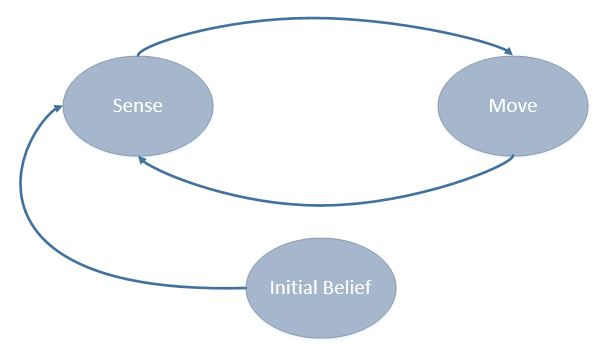
\includegraphics[scale=0.45]{images/SenseMoveInitialBelief}
\caption{Main tasks of localization}
\label{fig:main tasks}
\end{figure}

The first of the two tasks for the robot is to sense. This in done by using the sensors which are built in to the robot. As an example the robot could measure the distance to all walls in the environment or the color of the floor. These measurements should lead to a better belief of where the robot is located. Every time the robot senses it gains information of where it is located. The second task for the robot is to move. The robot needs to move in order to be able to get new information from the sensing task. When the robot moves it looses information of where it is located. This is due to inaccuracy of the robots speed and orientation. This will be illustrated in a robot example later on in this section.\\

The algorithm to implement the two tasks is called the Markov Localization algorithm and is illustrated in Algorithm \ref{alg:ml_def1}. The algorithm is based on the Bayes filter algorithm and calculates the new belief based on the old belief $bel(x_{(t-1)})$, the motion $u_t$, the measurements $z_t$ and the map.

\begin{center}
\begin{minipage}{.65\linewidth}
\alglanguage{pseudocode}
\begin{algorithm}[H]
\caption{Markov Localization}
\label{alg:ml_def1}
\begin{algorithmic}[1]
\Procedure{MarkovLocalization}{$bel(x_{t-1}),u_{t},z_{t},m$}
  \ForAll{$x_{t}$}
    \State $\overline{bel}(x_{t}) = \int{p(x_{t}|u_{t},x_{t-1},m)bel(x_{t-1})dx}$
    \State $bel(x_{t}) = \eta\;p(z_{t}|x_{t},m)\overline{bel}(x_{t})$
  \EndFor
  \State \textbf{return} $bel(x_{t})$
\EndProcedure
\end{algorithmic}
\end{algorithm}
\end{minipage}
\end{center}

The first step in the algorithm is line 3 in Algorithm \ref{alg:ml_def1}. In this line the algorithm calculates the sum of the product of two distributions. The two distributions are the prior belief of the robot being at the position $x_{t-1}$ and the probability that the motion $u_t$ moved the robot from the position $x_{t-1}$ to the new position $x_t$ according to the map. This step in the algorithm is referred to as the motion update. \\

The second step is line 4 in Algorithm \ref{alg:ml_def1}. This step looks at the probability that the measurement $z_t$ may have been observed at the the location $x_t$ according to the map. This is multiplied by the belief of $x_t$. This product is normalized by the normalization constant $\eta$ so it will integrate to 1. This step is referred to as the measurement update.\\

The algorithm needs a prior belief to calculate the new belief. If no initial belief is known the algorithm should use a uniform distribution as the prior belief.

\subsection{Robot Example} % (fold)
\label{sub:robot_example}

This is an example of the localization process where a robot has to localize itself. In \autoref{fig:initialBelief} the scenario is illustrated. The robot is in an environment with three doors. The robot has no idea of where it is located and the initial belief $bel(x)$ is therefore a uniform distribution.

\begin{figure}[H]
\centering
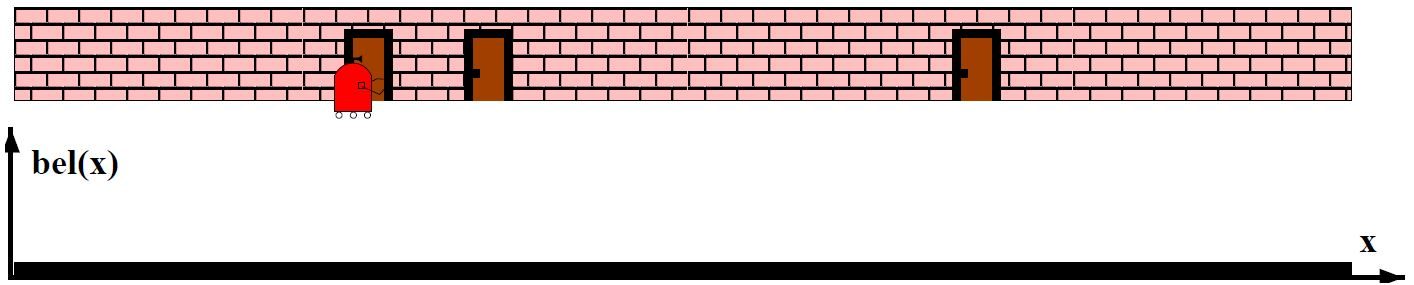
\includegraphics[scale=0.36]{images/MarkovLocalizationA}
\caption{The initial belief of the robot's location}
\label{fig:initialBelief}
\end{figure}

As the robot starts localizing itself it performs a sensing task. The measurement indicates that the robot is located next to a door. This measurement should only be obtained at three different locations in this environment. The probability of obtaining this measurement when located at those three locations, $p(z|x)$, therefore increases as illustrated in \autoref{fig:afterSenseBelief}. The new belief is calculated as the product of the prior belief and this probability.

\begin{figure}[H]
\centering
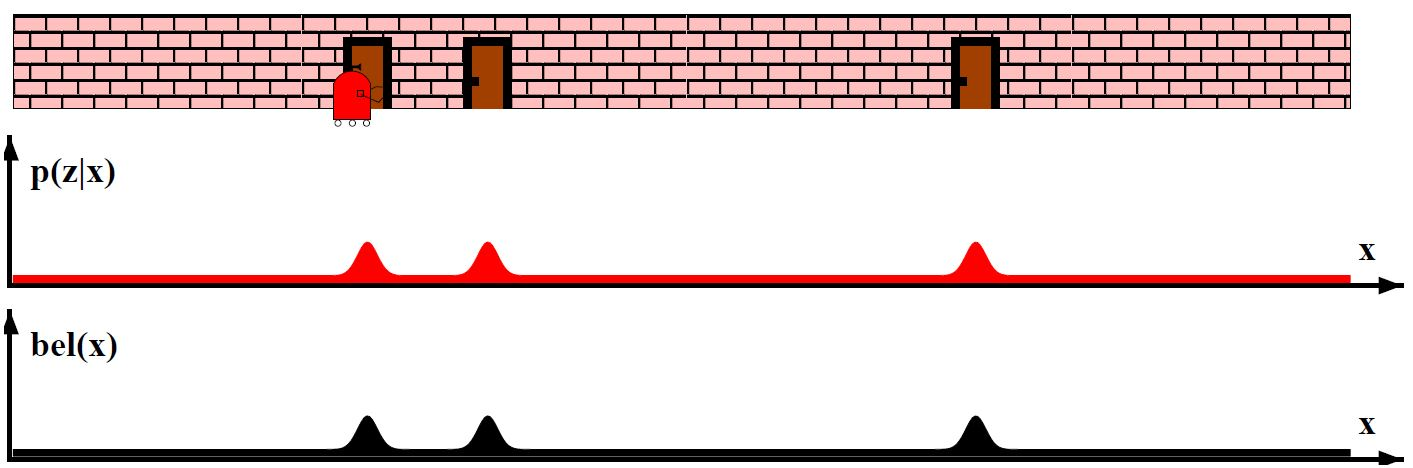
\includegraphics[scale=0.36]{images/MarkovLocalizationB}
\caption{The belief of the robot's location after sensing}
\label{fig:afterSenseBelief}
\end{figure}

The next task for the robot is the moving task. The robot moves a little to the right as illustrated in \autoref{fig:afterMoveBelief}. The belief is now a little less sure of the three most possible locations. This is due to inaccuracy as described earlier in this section.

\begin{figure}[H]
\centering
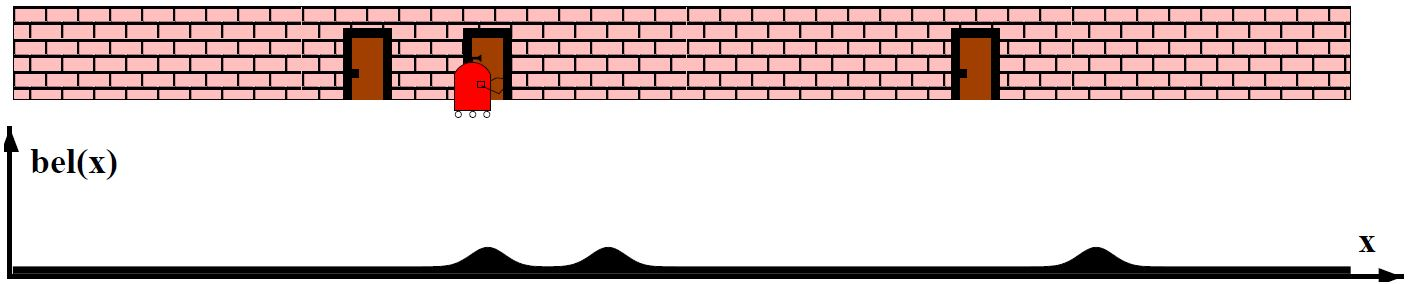
\includegraphics[scale=0.36]{images/MarkovLocalizationC}
\caption{The belief of the robot's location after moving}
\label{fig:afterMoveBelief}
\end{figure}

The robot performs a new sense task and the measurement indicated that the robot is located at a door which leads to a probability similar to the one obtained after the first sensing task. This time, as last time, it is multiplied by the prior belief. This results in a new belief with only one dominant location as illustrated in \autoref{fig:afterSecondSenseBelief}. 

\begin{figure}[H]
\centering
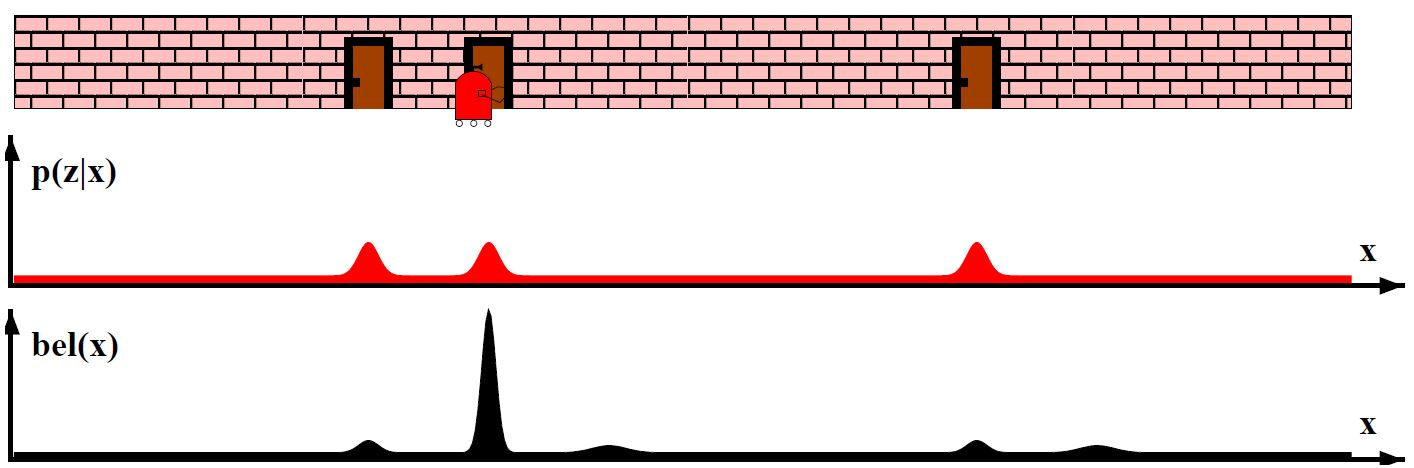
\includegraphics[scale=0.36]{images/MarkovLocalizationD}
\caption{The belief of the robot's location after second sensing}
\label{fig:afterSecondSenseBelief}
\end{figure}

Even though the robot moves the one location is still dominant as illustrated in \autoref{fig:finalBelief}. Hence only one location is dominant and the robot has now localized itself.

\begin{figure}[H]
\centering
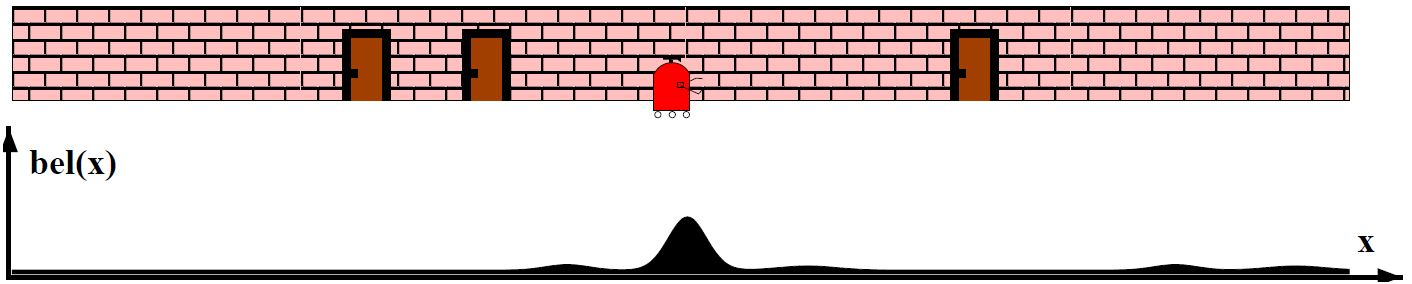
\includegraphics[scale=0.36]{images/MarkovLocalizationE}
\caption{The robot localizes itself}
\label{fig:finalBelief}
\end{figure}

% subsection robot_example (end)

% section localization (end)

%!TEX root = ../Master.tex

\section{Kalman filters}

The Kalman filter (KF) is a technique for filtering and prediction in linear systems. In the context of robotics the filter can be used to locate the robot and make predictions as to where the robot will reside in the next time-step.\\

The technique makes it possible to do data fusion, which is the process of combining observations from a number of different sensors to provide a robust and complete description of the environment. Robots could e.g. use radar, lidar, GPS, compass, camera, etc. for location and combining these sensor informations would result in are more complete overview of the robot and its environment.\\

The KF consists of a basic cycle which includes making predictions and updating these predictions with actual measurement data. The filter represents it's beliefs about state of the system as a Gaussian distribution which is characterized by two parameters: the mean value $\mu$ and the variance $\sigma^2$. Another important property of the KF and Gaussians is that they are unimodel. This means that they posses a single maximum as opposed to e.g. Particle Filters and Monte Carlo Localization which are multimodal.\\

The formal definition of the KF algorithm is given in Algorithm \ref{alg:kf_def1}. Notice that the variance is now represented by $\Sigma_{t}$ which in higher dimensional spaces denotes an covariance matrix.

\begin{center}
\begin{minipage}{.65\linewidth}
\alglanguage{pseudocode}
\begin{algorithm}[H]
\caption{Kalman Filter}
\label{alg:kf_def1}
\begin{algorithmic}[1]
\Procedure{KalmanFilter}{$\mu_{t-1},\Sigma_{t-1},u_{t},z_{t}$}
  \State $\bar\mu_{t} = A_{t}\mu_{t-1} + B_{t}u_{t}$%\Comment{This is a comment}
  \State $\bar\Sigma_{t} = A_{t}\Sigma_{t-1}A_{t}^T + R_{t}$
  \State $K_{t} = \bar\Sigma_{t}C_{t}^T(C_{t}\bar{\Sigma}_{t}C_{t}^T+Q_{t})^{-1}$
  \State $\mu_{t} = \bar\mu_{t} + K_{t}(z_{t} - C_{t}\bar\mu_{t})$
  \State $\Sigma_{t} = (I - K_{t}C_{t})\bar\Sigma_{t}$
  \State \textbf{return} $\mu_{t}, \Sigma_{t}$
\EndProcedure
\end{algorithmic}
\end{algorithm}
\end{minipage}
\end{center}

The algorithm takes four parameters: The previous mean value and variance of the system $\mu_{t-1}$ and $\Sigma_{t-1}$, respectively, the new control-input $u_{t}$ and measurement data $z_{t}$. In line 2 the previous mean value and control-input are mapped into the new mean value $\bar{\mu_{t}}$ which is a prediction of the system state. In line 3 the variance is propagated together with the measurement noise $R_{t}$. In line 4 the Kalman gain is calculated, which is used as a weight factor in line 5 to determine the degree to which we believe in the measurement as opposed to the prediction. Lastly the variance is updated in line 6.\\

The mean value of the system could be a position, velocity or a heading. The transition matrix $A_{t}$ applies the effects of $\mu_{t-1}$ on $\mu_{t}$, and the transition matrix $B_{t}$ applies the effects of control-input $u_{t}$ on $\mu_{t}$. The factors $R_{t}$ and $Q_{t}$ models the motion noise and measurement noise, respectively. In higher dimensional spaces these will be covariance matrices.\\

As mentioned, the KF represents its beliefs about the system, predictions and measurements, as Gaussians. An important property of the KF is that combining the predictions and the measurements increases the certainty about the system state. Gaussians has the characteristic that multiplying two Gaussians produces a new Gaussian with a variance that is smaller than the variance of both of the original Gaussians, and therefore this new Gaussian will have a larger peak than the original Gaussians. The mean value of the new Gaussian will lie between the two mean values of the two original Gaussians. \\

The measurement update consists of the multiplication of the prediction and the measurement Gaussians. The equations for the new mean value and variance of the Gaussian are given in equation \ref{eq:new_mu1} and \ref{eq:new_sigma1}, respectively.

\begin{equation}
\label{eq:new_mu1}
\mu = \dfrac{\sigma_{2}^2\mu_{1} + \sigma_{1}^2\mu_{2}}{\sigma_{2}^2 + \sigma_{1}^2}
\end{equation}
\begin{equation}
\label{eq:new_sigma1}
\sigma^2 = (\dfrac{1}{\sigma_{2}^2} + \dfrac{1}{\sigma_{1}^2})^{-1}
\end{equation}

There is a certain degree of error involved in the motion of an object due to e.g. friction. The motion update therefore consists of moving the mean value $\mu_{t-1}$ and adding some degree of uncertainty to the Gaussian which increases the variance of the new Gaussian w.r.t the original Gaussian. The motion update turns out to be very simple and is preformed by adding the mean values and variances of the Gaussians representing the posterior and priori beliefs. The equations for the motion update is giving in \ref{eq:new_mu2} and \ref{eq:new_sigma2}.

\begin{equation}
\label{eq:new_mu2}
\mu = \mu_{1} + \mu_{2}
\end{equation}
\begin{equation}
\label{eq:new_sigma2}
\sigma^2 = \sigma_{1}^2 + \sigma_{2}^2
\end{equation}

\subsection{Kalman Filter example}

A simple example of the KF in a one-dimensional location scenario is given in \autoref{fig:kf_ex}. A robot moves along the horizontal ax, and the initial belief about the robots location is shown in \autoref{fig:kf_ex}(a). The bold graph in \autoref{fig:kf_ex}(b) represents measurement data obtained from e.g. GPS or distance measurements relative to objects with a known location. In the measurement update step, the initial belief is combined with the measurements, which is a product of the two Gaussians. This improved belief about the robots location is calculated using equations \ref{eq:new_mu1} and \ref{eq:new_sigma1}. The result is the bold graph shown in \autoref{fig:kf_ex}(c). As mentioned, the mean value of this new Gaussian is located between the mean values of initial belief and the measurement and the variance of the new Gaussian is smaller than the variances of both the original Gaussians. In \autoref{fig:kf_ex}(d) the bold graph represents the prediction of the location of the robot which is calculated in line 2 of Algorithm \autoref{alg:kf_def1}. \\

In the motion update step, the robot is moved along the horizontal ax by adding some control-input value to the mean value of the robot, and because movement is prone to some amount of error, the variance is added with an error value to increase the variance representing the motion update uncertainty. The bold graph in \autoref{fig:kf_ex}(e) again represents a measurement made by the robot, which is combined with the prediction resulting in the bold graph in \autoref{fig:kf_ex}(f).

\begin{figure}[H]
\centering
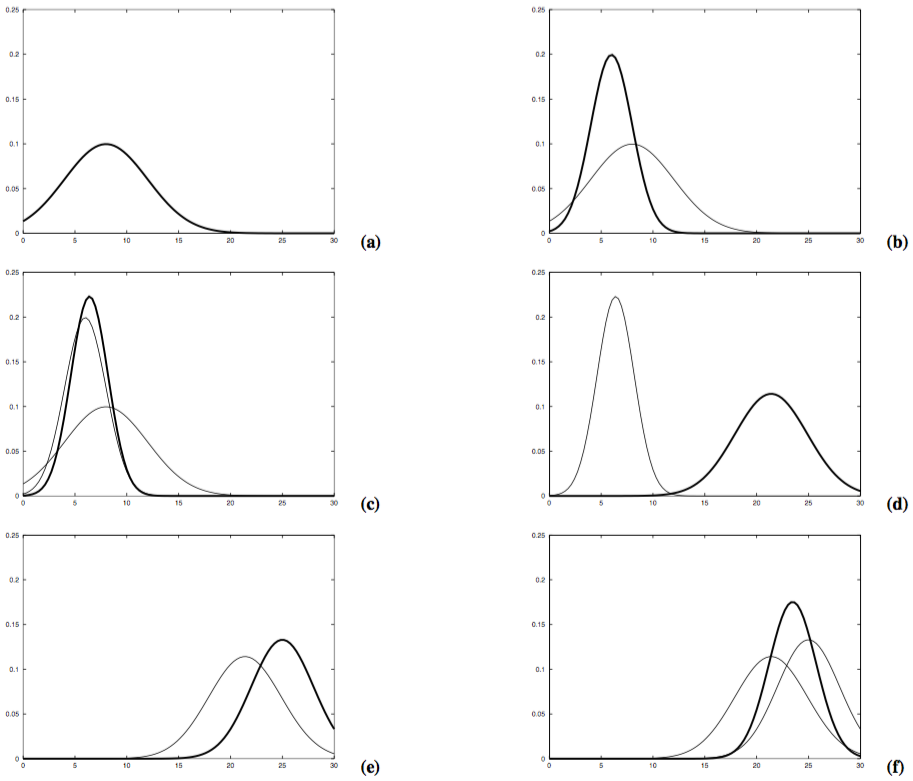
\includegraphics[scale=0.45]{images/KalmanFilterExample}
\caption{Kalman Filter example in a one-dimensional localization scenario}
\label{fig:kf_ex}
\end{figure}

\subsection{Extended Kalman filters}

The plain KF assumes that the system is linear in the state transitions and measurements with added Gaussian noise. This is however not the case in many systems and therefore the KF is inapplicable in many non-trivial problems.\\

To overcome this limitation of the plain KF, the extended Kalman Filter (EKF) can be used instead. In the EKF linearization is used to generate an approximation to the nonlinear system. This approximation to the true belief is represented by a mean value $\mu_t$ and a variance $\sigma_t^2$. Therefore the EKF represents its belief as the plain KF, but it uses an approximation instead of the exact belief.\\

The formal definition of the EKF is given in Algorithm \ref{alg:ekf_def1}.

\begin{center}
\begin{minipage}{.65\linewidth}
\alglanguage{pseudocode}
\begin{algorithm}[H]
\caption{Extended Kalman Filter}
\label{alg:ekf_def1}
\begin{algorithmic}[1]
\Procedure{ExtendedKalmanFilter}{$\mu_{t-1},\Sigma_{t-1},u_{t},z_{t}$}
  \State $\bar\mu_{t} = g(u_t,\mu_{t-1})$
  \State $\bar\Sigma_{t} = G_{t}\Sigma_{t-1}G_{t}^T + R_{t}$
  \State $K_{t} = \bar\Sigma_{t}H_{t}^T(H_{t}\bar{\Sigma}_{t}H_{t}^T+Q_{t})^{-1}$
  \State $\mu_{t} = \bar\mu_{t} + K_{t}(z_{t} - h(\bar{\mu_t}))$
  \State $\Sigma_{t} = (I - K_{t}H_{t})\bar\Sigma_{t}$
  \State \textbf{return} $\mu_{t}, \Sigma_{t}$
\EndProcedure
\end{algorithmic}
\end{algorithm}
\end{minipage}
\end{center}

The EKF in Algorithm \ref{alg:ekf_def1} looks very similar to the plain KF in Algorithm \ref{alg:kf_def1}. But the important difference are seen in line 2 and line 5, where the linear prediction of the KF are replaced by the linearized functions $g(u_t,\mu_{t-1})$ and $h(\bar{\mu_t})$, respectively. Also, the linear system matrices $A_t$ and $B_t$ have been replaced with the Jacobian $G_t$, and $C_t$ with $H_t$. The Jacobians are a consequence of the linearized operation.

%!TEX root = ..\Master.tex

\section{Particle Filters}
%!TEX root = ../Master.tex

\section{Path Planning} % (fold)
\label{sec:path_planning}

When a robot has located itself the next task might be to go somewhere. The task of planning a path from the location of the robot to some goal location is, when talking about robots, often referred to as robot motion planning. The problem to solve is to find the best possible path for the goal location when knowing the start location, the map and maybe some kind of cost function. This cost function can be thought of as the time it takes to follow a certain route. When introducing this cost function the best possible path is the minimum cost path. \\

\subsection{A* Algorithm} % (fold)
\label{sub:a_algorithm}

The path planning can be looked at as a search problem. A search problem is a problem with a set of nodes, an initial node and a goal node. The search problem can be solved by using a search algorithm. The search algorithm starts at the initial node and searches throughout the nodes in order to find the goal node. A variant of this search algorithm has been developed in order to handle the problem of path planning better. This algorithm is referred to as A* (pronounced A star). The steps of the algorithm is explained in the following section. \\

To understand the approach of the A* algorithm a couple of variables must be introduced.

\begin{itemize}
	\item The \emph{g} value is the cost of the path used to get to that node.

	\item The \emph{h} value is the number of nodes to pass to get to the goal node without taking obstacles into account. This can also be looked at as the displacement along both the x-axis and the y-axis of a node compared to the goal node.

	\item The \emph{f} value is the sum of the \emph{g} value and the \emph{h} value.\\
\end{itemize}

The algorithm also introduces three different lists.

\begin{itemize}
	\item The \emph{open} list is a list of nodes to be investigated. The list is sorted so that the node with the smallest \emph{f} value is the next node to be investigated. Nodes are being added to the \emph{open} list when a neighbor node is being investigated.

	\item The \emph{closed} list is a list of all nodes which have been investigated. This is used to keep track of these nodes in order to avoid investigation of a node twice or more.

	\item The \emph{action} list is a list which keeps track of which node was the previous node for all investigated nodes.\\
\end{itemize}

The procedure of the algorithm is as following. 

\begin{enumerate}
  \item The initial node is added to the \emph{open} list.

  \item The node in the \emph{open} list with the lowest \emph{f} value is chosen to be investigated. The chosen node is deleted from the \emph{open} list and added to the \emph{closed} list. 

  \item All neighbor nodes which are not in the \emph{closed} list are added to the \emph{open} list. All nodes are added to the \emph{action} list together with the information of which node was the previous node.
\end{enumerate}

Step two and three are repeated until the node from the \emph{open} list is the goal node. Then the planned path can be found. This is done by introducing a new list called \emph{path}. The goal node is added to this list and from the \emph{action} list the previous node is known. This node is added to the \emph{path} list. The previous node to this node is looked up in the \emph{action} list and so on until the previous node is the initial node. After reversing the \emph{path} list the path for the robot is planned. \\

% subsection a_algorithm (end)

\subsection{Path Smoothing} % (fold)
\label{sub:path_smoothing}

As described the A* algorithm results in a \emph{path} list. This planned path might be a very cornered path with lots of sharp turns for the robot to do. If this is not desirable for the robot the path can be smoothed. \\

For the smoothing algorithm all nodes in the \emph{path} list are denoted $x_i$ where $i$ is the number the node has in the list. All nodes in the \emph{smoothened path} list is denoted $y_i$. The algorithm has to solve a minimization problem. The \emph{smoothened path} list is initialized to be the same as the \emph{path} list as it is denoted in \autoref{eq:init_smooth_path}.

\begin{equation}
\label{eq:init_smooth_path}
y_i = x_i
\end{equation}

The minimization problem is defined in \autoref{eq:minimize}. The factor $\alpha$ sets how smooth the path is going to be. The larger value of $\alpha$, the more smooth the path gets. 

\begin{equation}
\label{eq:minimize}
\text{minimize\ } (x_i - y_i)^2 - \alpha (y_i - y_{i+1})^2
\end{equation}

In an implementation of the path smoothening algorithm two values are used to regulate for the smoothening, $\alpha$ and $\beta$. The $\alpha$ value yields how much the path should smoothen and the $\beta$ value yields how much the path should look like the original path. The path is being changed until the new change is smaller than some tolerance. An example of an implementation is shown in \autoref{smooth_path}. Notice that when the algorithm is implemented the initial node and the goal node has to stay unchanged.

\begin{lstlisting}[caption=Implementation example of path smoothing., label=smooth_path, language=Matlab]
function newpath = smoothPath(path, alpha, beta, tolerance)
    [length, width] = size(path);
    newpath = zeros(length,width);
    
    for i = 1:length
        for j = 1:width
            newpath(i,j) = path(i,j);
        end
    end
    
    change = tolerance;
    while change >= tolerance
        change = 0;
        for n = 2:length - 1
            for m = 1:width
                aux = newpath(n,m);
                newpath(n,m) = newpath(n,m) + alpha * (path(n,m) - newpath(n,m));
                newpath(n,m) = newpath(n,m) + beta * (newpath(n-1,m)+newpath(n+1,m)-2*newpath(n,m));
                change = change + abs(aux - newpath(n,m));
            end
        end
    end
end
\end{lstlisting}

% subsection path_smoothing (end)
% section path_planning (end)
%!TEX root = ..\Master.tex

\section{PID Control}
%!TEX root = ../Master.tex

\section{SLAM}

A fundamental problem involved with AI in robotics is localization and mapping. This problem arises when the robot does not have a map of the environment and do not know it's pose. Usually the only information the robot have at it's disposal are measurements and control-inputs. This problem is commonly referred to as \textit{Simultaneous Localization And Mapping} abbreviated or \textit{SLAM}.\\

A technique to solve the SLAM problem is called GraphSLAM. As the name suggest, this technique represents the robots poses and landmarks as nodes in a graph and constraints between poses, resulting from measurements, are encoded on the edges between nodes. An edge between two nodes therefore represents a spatial constraint relating the two robot poses. Since constraints are generated from measurements which we represent as Gaussians because of measurement uncertainty, the goal then, is to find a configuration of the nodes that minimize the error introduced by the constraints.\\

We represent the constraints between poses and landmarks using a matrix $\Omega$ and a vector $\xi$. The matrix describes which object (poses and landmarks) in the environment that are related, and the vector contains a value for this relationship which could be a distance between the objects. When new constraint are generated by the robot, the matrix and vector is modified by adding the constraints to a subset of the matrix and vector.\\

Once the constraints have been defined in the matrix and vector pair, the best estimate of the robot poses and landmarks positions can be calculated by inverting the matrix $\Omega$ and multiplying it with the vector $\xi$ as shown by Equation \ref{eq:slam_est}.

\begin{equation}
\label{eq:slam_est}
\mu = \Omega^{-1}\xi
\end{equation}

To summarize, in the graph-based SLAM technique, we add information to the matrix $\Omega$ and vector $\xi$ every time an constraint is encountered, and when we are done gathering constraints a simple procedure is run which gives the robot poses and landmark locations.

\subsection{GraphSLAM example}

In this section a simple example is given on how to use GraphSLAM which involves defining constraints and solving a system of equations to obtain robot and landmark locations.\\

Given the graph in \autoref{fig:slam_ex} which shows three robot poses and a landmark, we need a matrix of size $4\times4$ and a vector of size 4 to describe all the constraints. The initial position of the robots is $x_0 = -3$ and we can define the local constraints of movement $x_0 \rightarrow x_1$ and $x_1 \rightarrow x_2$ as Equation \ref{eq:slam_pose_rel1_a} and \ref{eq:slam_pose_rel1_b}, respectively.

\begin{equation}
\label{eq:slam_pose_rel1_a}
x_1 = x_0 + 5
\end{equation}

\begin{equation}
\label{eq:slam_pose_rel1_b}
x_2 = x_1 + 3
\end{equation}

Which gives constraints in Equation \ref{eq:slam_pose_rel2_a} - \ref{eq:slam_pose_rel3_b}.

\begin{equation}
\label{eq:slam_pose_rel2_a}
x_0 - x_1 = -5
\end{equation}

\begin{equation}
\label{eq:slam_pose_rel2_b}
x_1 - x_0 = 5
\end{equation}

\begin{equation}
\label{eq:slam_pose_rel3_a}
x_1 - x_2 = -3
\end{equation}

\begin{equation}
\label{eq:slam_pose_rel3_b}
x_2 - x_1 = 3
\end{equation}

Adding constraints in Equation \ref{eq:slam_pose_rel2_a} and \ref{eq:slam_pose_rel2_b} together with the initial position of the robot, gives the matrix and vector shown in Equation \ref{eq:slam_matrix1}.

\begin{equation}
\label{eq:slam_matrix1}
\begin{bmatrix}
2 & -1 & 0 & 0 \\
-1 & 1 & 0 & 0 \\
0 & 0 & 0 & 0 \\
0 & 0 & 0 & 0 \\
\end{bmatrix}
\begin{bmatrix}
-8 \\
5 \\
0 \\
0 \\
\end{bmatrix}
\end{equation}

Adding the constraint relating $x_1$ to $x_2$ results in the matrix and vector shown in Equation \ref{eq:slam_matrix2}.

\begin{equation}
\label{eq:slam_matrix2}
\begin{bmatrix}
2 & -1 & 0 & 0 \\
-1 & 2 & -1 & 0 \\
0 & -1 & 1 & 0 \\
0 & 0 & 0 & 0 \\
\end{bmatrix}
\begin{bmatrix}
-8 \\
2 \\
3 \\
0 \\
\end{bmatrix}
\end{equation}

Now the constraints relating the robot poses is added to the landmark.

\begin{figure}[H]
\centering
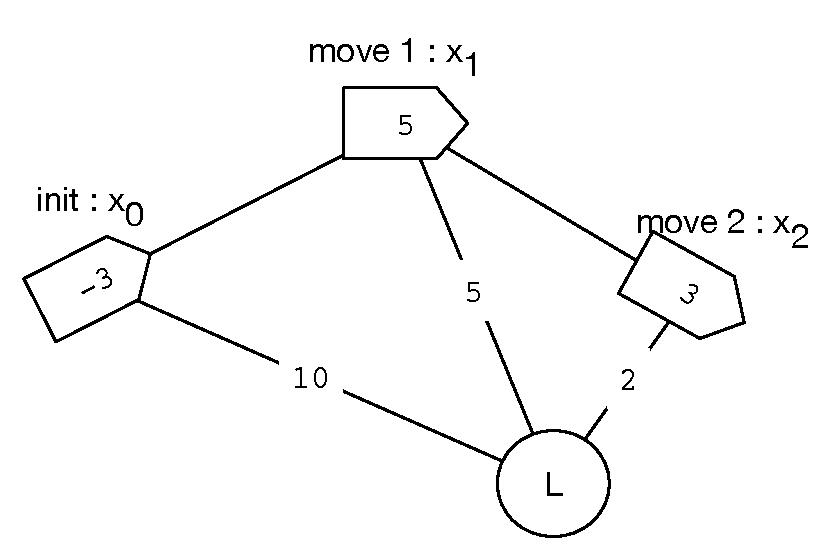
\includegraphics[scale=0.70]{images/ex_slam_graph}
\caption{GraphSLAM example}
\label{fig:slam_ex}
\end{figure}

The relation between the three poses and the landmark is giving by Equation \ref{eq:slam_lan_rel1} - \ref{eq:slam_lan_rel3}.

\begin{equation}
\label{eq:slam_lan_rel1}
L = x_0 + 10
\end{equation}

\begin{equation}
\label{eq:slam_lan_rel2}
L = x_1 + 5
\end{equation}

\begin{equation}
\label{eq:slam_lan_rel3}
L = x_2 + 2
\end{equation}

Which gives the constraints for $x_0 \rightarrow L$.

\begin{equation}
\label{eq:slam_lan_cons1_a}
x_0 - L = -10
\end{equation}

\begin{equation}
\label{eq:slam_lan_cons1_b}
L - x_0 = 10
\end{equation}

And for $x_1 \rightarrow L$.

\begin{equation}
\label{eq:slam_lan_cons2_a}
x_1 - L = -5
\end{equation}

\begin{equation}
\label{eq:slam_lan_cons2_b}
L - x_1 = 5
\end{equation}

And lastly for $x_2 \rightarrow L$.

\begin{equation}
\label{eq:slam_lan_cons3_a}
x_2 - L = -2
\end{equation}

\begin{equation}
\label{eq:slam_lan_cons3_b}
L - x_2 = 2
\end{equation}

Adding these constraints to the matrix and vector in Equation \ref{eq:slam_matrix2} produces the matrix and vector in Equation \ref{eq:slam_matrix3}.

\begin{equation}
\Omega =
\label{eq:slam_matrix3}
\begin{bmatrix}
3 & -1 & 0 & -1 \\
-1 & 3 & -1 & -1 \\
0 & -1 & 2 & -1 \\
-1 & -1 & -1 & 3 \\
\end{bmatrix}\,
\xi =
\begin{bmatrix}
-18 \\
-3 \\
1 \\
17 \\
\end{bmatrix}
\end{equation}

Solving this system using Equation \ref{eq:slam_est} produces the best estimate $\mu$ shown in Equation \ref{eq:slam_calc}.

\begin{equation}
\label{eq:slam_calc}
\mu = \Omega^{-1}\xi = 
\begin{bmatrix}[2.2]
1 & 1 & 1 & 1 \\
1 & \dfrac{13}{8} & \dfrac{3}{2} & \dfrac{11}{8} \\
1 & \dfrac{3}{2} & 2 & \dfrac{3}{2} \\
1 & \dfrac{11}{8} & \dfrac{3}{2} & \dfrac{13}{8} \\
\end{bmatrix}
\begin{bmatrix}[2.2]
-18 \\
-3 \\
1 \\
17 \\
\end{bmatrix} =
\begin{bmatrix}[2.2]
-3 \\
2 \\
5 \\
7 \\
\end{bmatrix}
\end{equation}

Meaning that the positions of the robot and the landmark are $x_0 = -3$, $x_1 = 2$, $x_2 = 5$, and $L = 7$. Note that in Equation \ref{eq:slam_matrix3} matrix $\Omega$ has zeros in positions $\Omega_{3,1}$ and $\Omega_{1,3}$ meaning that there is no constraint between $x_0$ and $x_2$. This can also be seen in \autoref{fig:slam_ex} by the absence of an edge between these two nodes.


\chapter{Project}
%!TEX root = ../Master.tex

\section{Introduction} % (fold)
\label{sec:prokect_introduction}

This chapter describes the projectwork carried out as part of the course AI In Robotics. The aim of the project is to apply the theory learned during the course by implementing the algorithms and methods and simulating and/or executing the result on some robot platform.\\
In this project the main focus have been on the software implementations of the theory, and the hardware concerns have been given a lower priority made possible by using a hardware platform running a robot operating system (ROS) that provides high-level abstractions for execution of control-inputs and obtaining measurements data.\\

Hardware, software, simulation, and test will be described in greater detail in the subsequent sections, and we give a discussion about our results ending with a conclusion of the project.

% section introduction (end)
%!TEX root = ../Master.tex

\section{Hardware} % (fold)
\label{sec:hardware}

As mentioned in \autoref{sec:prokect_introduction} the focus of the project have been on the software implementations of theory learned throughout the course. By using a Neato XV-11 vacuum cleaning robot in \autoref{fig:neato_xv11} which have a build-in lidar to sense its environment, and that implements functionality to move by some unit distance, most hardware concerns have been eliminated.\\

\begin{figure}[H]
\centering
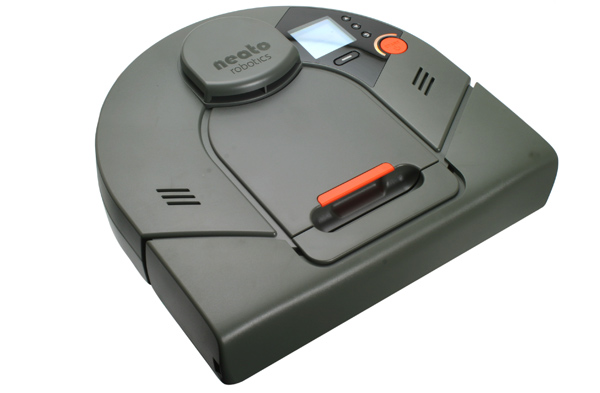
\includegraphics[scale=0.40]{images/neato_xv11}
\caption{Neato XV-11}
\label{fig:neato_xv11}
\end{figure}

The lidar is also developed by Neato and ...\\
\fxnote{Add facts about lidar, and maybe other things about the robot hardware.}

The Neato robot runs ROS which makes it possible to develop and simulate the robot on a PC, and the code can then to loaded onto the robot and executed.\\
However, there are some discrepancies between simulation and real-life execution regarding lidar measurements, which have hindered testing on the actual robot.

% section hardware (end)
%!TEX root = ../Master.tex

\section{Software} 
\label{sec:software}

The software was written mostly in c++ for its speed and partly in python for easy integration with an existing driver for the neato robot. ROS (Robot Operating System) was used for visualization and communication.

\subsection{ROS}
To be able to easily test and validate the implemented AI methods, we used ROS to visualize the system. ROS  is a collection of software for building robot systems and has a large collection of packages for 3D visualization, navigation, mapping, localization, planning, etc. Only the visualization and communication parts of ROS has been used in this project. This is chosen due to the purpose of trying to implement localization, planning and control ourself. \\

A ROS project consists of a collection of processes with a single responsibility, i.e. planning, vision, control, etc. ROS also handles the communication between these processes. The processes are conceptualized as nodes in a network which can communicate by publishing and subscribing on topics. \\

The communication in ROS consists of messages with a specific data type. The data type could be anything from simple integers to LaserScans which describes a scan from a lidar and extra header information as a time stamp and a sequence number if the order of scans are important. A node can also contain services which can be called with a request-response communication model, instead of the the publish-subscribe model between nodes.\\

ROS master is the program that coordinates the communication between the nodes. It also works as a registry for nodes, services, topics, etc.

\subsubsection{ROS Nodes}
The system implements two ROS nodes, the first is a driver for Neato robot and the second is the navigation system.\\

The driver is a modified version of an open source driver for the robot. \fixme{\cite{neatoGithub}} The open source driver implements an older version of the serial protocol for the Neato robot. This has been modified to implement the newer protocol which the used robot uses.\\

The navigation node implements all of the AI algorithms; localization, planning and control. The two nodes communicate using ROS messages for lidar scans and control commands. 

\subsection{Neato driver node}
The neato driver node subscribes on the "command" topic to get the motion commands from the navigation node. After executing the motion command the node publishes the latest laser scan to the navigation node. This way the navigation node will always get a laser scan from the new position of the robot.

\subsection{Navigation node}
Most of the work has been in the navigation node where localization, planning and control is implemented. When a laser scan is received from the robot, a calculation of the next motion command is initialized. The Monte Carlo localizer is used to get an estimate of the current position. The uncertainty of the estimate is used to determine whether to trust it and follow a path to the goal or to keep driving around the map to decrease the uncertainty of the estimate. \autoref{fig:diagram} shows a class diagram for the navigation software. Each class is explained in more detail in the following sections.

\begin{figure}[H]
\centering
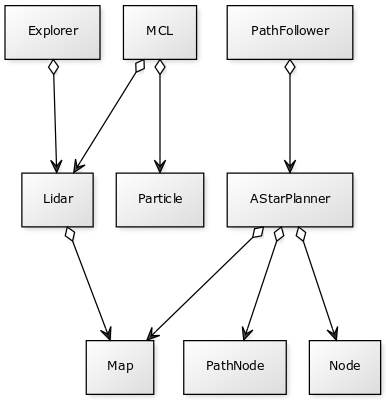
\includegraphics[scale=0.40]{images/diagram}
\caption{Class diagram for control and localization program}
\label{fig:diagram}
\end{figure}

\subsubsection{Map}
The map is implemented as a matrix of grid cells where each grid cell represents a $25cm\times25cm$ square in the real world. Each grid cell consists of an integer describing what is in the grid cell. For instance every cell describing a wall has the value 100, open floor is 20, the preferred path of the robot is 1. These specific values are chosen for use as a cost map for the path planning as they describe the cost of driving in that specific area. The map is also used when simulating lidar scans.

\subsubsection{Lidar}
The localization require the ability to simulate a lidar scan in the given map. This is implemented using a ray casting algorithm. Hence this was not part of the course curriculum, an open source implementation has been used. The class can calculate the distance from a given point on the map to the nearest wall in a given direction.

\subsubsection{Monte Carlo Localizer}
The localization in the project is implemented using the Monte Carlo localization algorithm. Initially all the particles are randomly spread across the map using a uniform distribution. This means that particles will be inside walls and in non-accessible areas, but the first re-sampling will move these particles to more likely positions.\\

Each time a lidar scan is received from the robot, the weight of each particle is updated. The weights are calculated using the lidar scan from the robot and a simulated scan from the Lidar class using the particles pose.
A Gaussian is used to model the error in sensor measurements, the variance is proportional to the simulated measurement to accommodate for a larger error over longer distances. For re-sampling the low variance re-sampler is used. This algorithm is shown in \autoref{fig:low_variance}.\\

\begin{figure}[H]
\centering
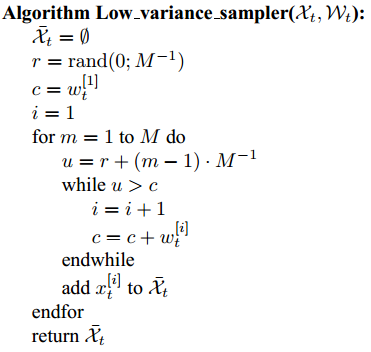
\includegraphics[scale=0.40]{images/low_variance_resampler}
\caption{Low variance re-sampler}
\label{fig:low_variance}
\end{figure}

Re-sampling happens after every 10th motion command. To get an estimate for the robots pose from all the particles, the particle with the highest weight is used. As a metric for the uncertainty of the estimate the variance of the particles is used.

\subsubsection{Explorer}
This class is used for calculating motion commands when the estimate uncertainty is high. It uses the lidar scan to look for obstacles and avoid them, while exploring as far away from its start position as possible. If nothing is in front of the robot, it will drive straight ahead. It looks at the measurements in front of the robot and if any of them are short it means an obstacle is ahead and it will do a 90 degree turn. It also looks for obstacles to the sides and turns to the free direction. If possible it will turn alternately 90 degrees left and right at each obstacle to avoid driving in circles. 

\subsubsection{PathFollower}
This class is used for calculating motion commands when the estimate uncertainty is low. It will use the AStarPlanner class to plan a path from the estimated position to a hard coded goal on the map. The path is a list of (x,y) points on the map. It will aim for the nearest point on the path and when it is close enough within some threshold it will start aiming for the next point.

\subsubsection{AStarPlanner}
This class implements the A* algorithm to do path planning. The different values of map are used as a cost-map to plan the best path.

%!TEX root = ../Master.tex

\section{Simulation} % (fold)
\label{sec:simulation}

RVIZ.
include images of 3D follower and top-down.
Explain what we see.
Explain the usefullness of the graphical feedback.


% section simulation (end)

%!TEX root = ../Master.tex

\section{Test} % (fold)
\label{sec:test}

% section test (end)
%!TEX root = ../Master.tex

\section{Discussion} % (fold)
\label{sec:discussion}

This section will discuss how the project could be improved to get better results.

\subsection{Localization}
One can't ensure that the particle filter will always find the correct position of the robot.
One way to improve our implementation is to use a better resampling strategy.
We resample at every 10 movements, which is a very simple strategy.
Our map has a lot of long straight coridors which all looks the same with a lidar range scan, so by resampling often while having particle clouds in multiple of these coridors, we might lose the cloud at the correct position.
This is because the weight of all the particles in the different coridors are about the same.
If we only resample when the variance in the particle weights are high we could maybe make the localization better. \\

Even with the above mentioned method, we cant be sure that the localization works everytime.
The augmented MCL algorithm could be used to recover from these failures.
The algorithm keeps track of the average weights on a long term and short term.
The lower the short term average weight is in relation to the long term average weight, the more particles are sampled randomly instead of from the existing particles.
The intuition is that when the average weight drops, it is because the particles no longer fits the correct position well, and we start probing the map at random for better positions. \\

The augmented MCL algorithm is a reactive algorithm in the sense that it reacts to the failure and tries to correct it.
The mixture MCL is a proactive method that should work even better.
During resample it will take a small amount of particles and place them at positions where the particle will get a high weight.
It basicly probes some of the likely positions on the map.
This way you reduce the risk of getting stuck with all the particles at a wrong position.

\subsection{Real robot}
We didn't get far while testing with the real robot even though the simulation worked much better.
One of the main issues was that we only model sensor noise as a normal distribution around the simulated measurement.
This way we don't handle the possiblity of corrupt measurements.
The Neato robot will give a sensor measurement of 0 when a measurement is invalid, and these should be ignored.
During testing we did not ignore these corrupt measurements.
We could also do tests to measure the variance of the noise on the real sensor and the variance of the execution of motion commands to get a better model of the real robot.

\subsection{ROS navigation stack}
ROS has open source packages for navigation, planning, control and mapping, which might work better than our implementations.

% section discussion (end)

%!TEX root = ../Master.tex

\section{Conclusion} % (fold)
\label{sec:conclusion}

The implementation of this project and this report has partly been a success.\\

Throughout the writing of the six summaries of the theory from this reading course a much better understanding of the theory has been obtained.\\

This has been a great basis for the attempt to implement the theory in a practical problem. This implementation worked most of the time in simulations but unfortunately this did not get to be carried out in a real-life problem.
% section conclusion (end)

%----------------------------------------------------------------------------------------
%	REFERENCE LIST
%----------------------------------------------------------------------------------------
\bibliography{bibtex/references}

%----------------------------------------------------------------------------------------

\end{document}